\begin{appendix}
\section{Matsubara Frequencies and Fast Fourier Transform}
In order to solve the impurity model we have to perform several Fourier Transform.
As we consider electrons, the Green's function in imaginary time is antiperiodic by shifts of $\beta$, so we have to use fermionic Matsubara frequencies $ω_n:=\frac{π(2n+1)}{β}$.
The Fourier Transformations are given by:

\begin{align}
  G(i ω_n) &:= \int_0^β dτ G(τ) e^{i ω_n τ}\\
  G(τ) &= \frac{1}{β} \sum_{i ω_n} G(i ω_n) e^{-i ω_n τ}
\end{align}
For effient calculations we use the FFT-algorithm of the numpy package. Therefore we have to adapt our definitions to the implementation of the numpy library. The numpy library calculates its Fourier Transform by:
\begin{equation}
  A_k = \mathrm{FFT}(a_m) =  \sum_{m=0}^{n-1} a_m \exp\left\{-2\pi i{mk \over n}\right\}
   \qquad k = 0,\ldots,n-1.
\end{equation}
Hence, we discretize the Matsubara Fourier transformation
\begin{align}
  G(i ω_{-n}) &\approx \sum_{k=0}^{N-1} \Delta τ \, G(\Delta τ \, k) \exp{\left(i \frac{π (-2n+1)k}{N}\right)}\\
          &=\frac{\beta}{N} \sum_{k=o}^{N-1} \left( G(\Delta τ \, k)\exp{\left(i π \frac{k}{N}\right)}  \right)  \exp{\left(i \frac{-2 π n k}{N}\right)}\\
	  &= \frac{\beta}{N} \mathrm{FFT}\left( G(\Delta τ \, k)\exp{\left(i π \frac{k}{N}\right)}\right), \label{eq:MFFT}
\end{align}
where $\Delta τ = \frac{\beta}{N}$.
The same can be carried out for the inverse Fourier Tranformations.
\begin{align}
	G(\Delta τ k) &= \frac{N}{β} e^{-i π \frac{k}{N}}\frac{1}{N}\sum_{ω_n}G(i ω_{-n}) e^{i 2π n k/N}\\
	&= \frac{N}{β} e^{-i π \frac{k}{N}}\mathrm{IFFT}(G(iω_{-n})) \label{eq:IMFFT}
\end{align}
\begin{figure}[h]
	\centering
	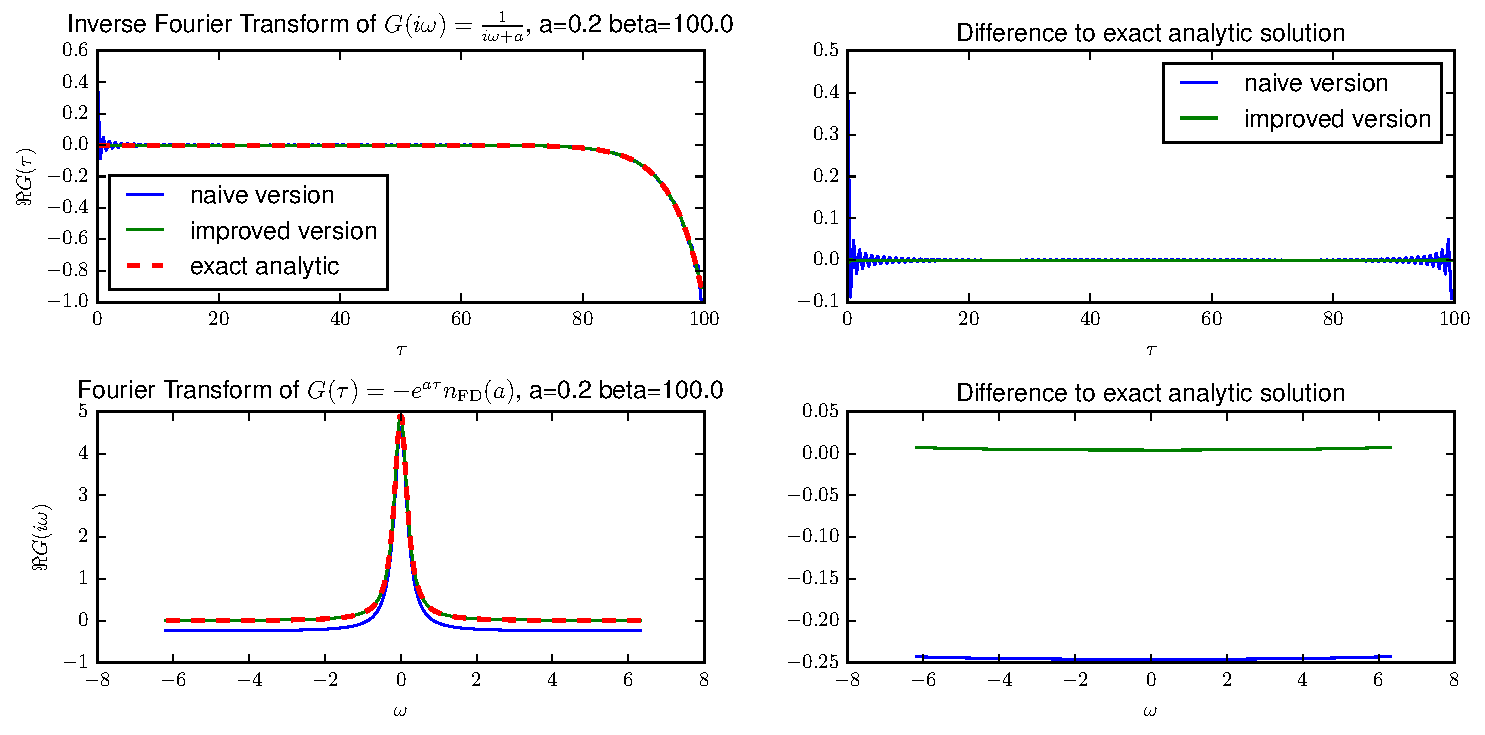
\includegraphics[width=\textwidth]{Matsubara_Fourier_fig}
	\caption{Comparison of the different discretized Fourier Transformations. The improved version, by manually removing the $\frac{1}{i \omega}$ factor, approximates the exact transformation significantly better. }
	\label{fig:fourier_traf}
\end{figure}
Unfortunately the ``naiv'' implementations \eqref{eq:MFFT} and \eqref{eq:IMFFT} cause numerical problems, since a typical Green's function in frequency space is of the form
\begin{equation}
	G(iω_n) = \frac{1}{iω_n +a} = \frac{1}{i ω_n} + \mathcal{O}\left(\frac{1}{ω_n^2}\right).
	\label{eq:expansion}
\end{equation}
Although $a$ can also be frequency dependent, the first term in the expansion of $G$ is always of the form as in \eqref{eq:expansion}.\todo{more details here?} Carrying out the sum over frequencies of this first term does unfortunately not converge, which is why we have to transform the $\frac{1}{i ω_n}$ part manually. %more information here?
From analytical calculation the Fourier transform is given as:
\begin{equation}
	G(τ)=-\frac{1}{2} \quad ⇔ \quad G(i ω_n) =\frac{1}{i ω_n}
	\label{eq:ff_pair}
\end{equation}
Consequently the improved version of our Fourier transformation is given by subtracting and adding the relevant terms before and after the transformation.
\begin{align}
	G(i ω_{-n})&= \frac{1}{i ω_{-n}}+\frac{\beta}{N} \mathrm{FFT}\left( \left(G(\Delta τ \, k)+\frac{1}{2}\right)\exp{\left(i π \frac{k}{N}\right)}\right)\\
	G(\Delta τ k)&= -\frac{1}{2}+\frac{N}{β} e^{-i π \frac{k}{N}}\mathrm{IFFT}\left(G(iω_{-n})-\frac{1}{i ω_{-n}}\right)
	\label{eq:improved_fft}
\end{align}
The improvement can be seen in \figref{fig:fourier_traf}, where we compare the exact Fourier transformation of $G(i ω)=\frac{1}{iω+a}$ to our discretized versions. The naiv version shows significant deviations to the analytic solution, whereas our improved version approximates the exact one very well.  


\section{Analytic continuation}
\begin{figure}[htb]
  \begin{center}
    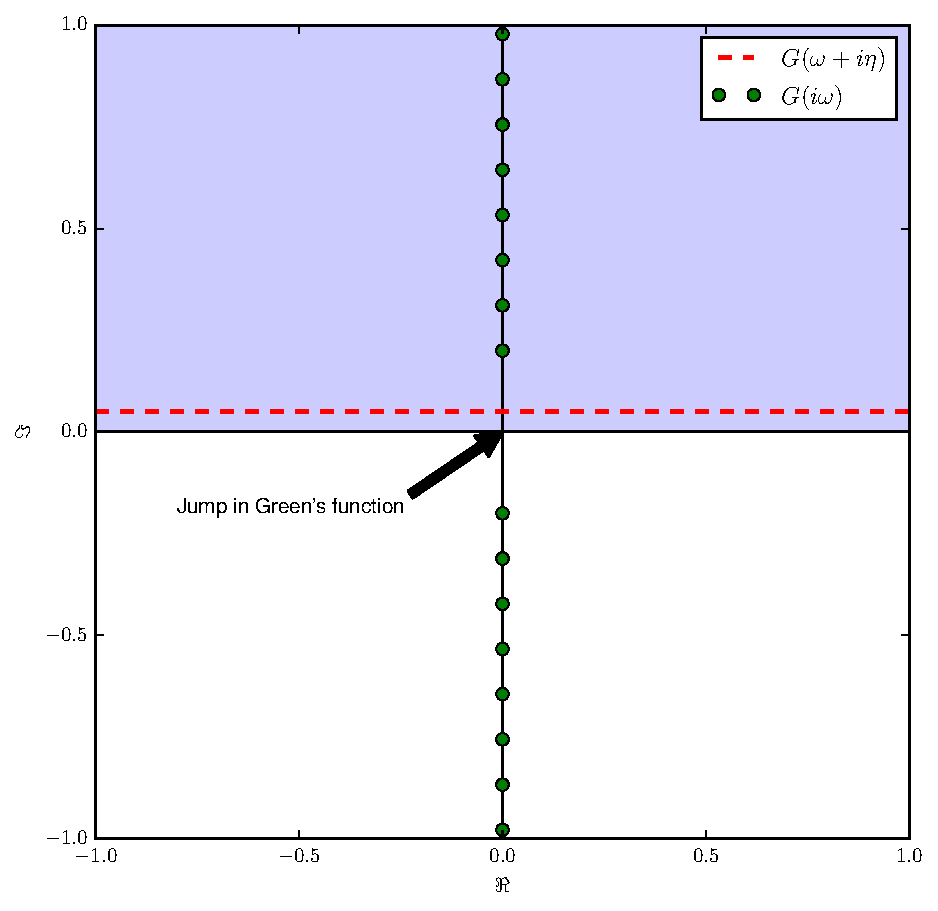
\includegraphics[width=0.7\textwidth]{analytic_continuation}
  \end{center}
  \caption{As the retarded Green's function (red) lies slightly above the real axis and the Matsubara Green's function shows discontinous jumps at zero frequency, we only take the postive frequencies to calculate the Padé approximation. Assuming that the Green's function is analytic in the upper half plane (blue), we expect the anayltic continuation with the rational function to approxmate the retarded Green's function both for positive and negative frequencies. }
  \label{fig:analytic_continuation}
\end{figure}


In order to calculate the spectral function $A$, we have to perform the anlytic continuation of the Matsubara Green's function.
This is a hard problem as we need the functional dependence of $G(iω_n)$ and the only information available is given by discrete points on the imaginary axis.
The central idea is now to interpolate our discrete points by a rational function, called Pade approximation, and use this function to do the analytic continuation. 
An efficient algortihm to calculalte the Padé approximation can be found in \cite{padepaper}. However, as the Padé approximation is continous, whereas the Green's function exhibits non-continous jumps, we have to think about, which values to use for the fit.

In the results of the DMFT-loop we observed discontinous jumps in the Matsubara Green's function at zero frequency.
As we exspect the Greens function to behave non-analytically only on the real axis, we can restrict ourselves on the positive or on the negative frequencies to calculate the fit and use the symmetry of the Greensfunction $G(iω)=G(-iω)^*$ to calculate its values on the opposite half plane.

Since the retared Green's function given by $G(i ω \to w + i o^+)$ lies slightly above the real axis, we can use the positive freqencies on the imaginary axis to calculate the fit and perform the analytic continuation both for positive and negative frequencies of the retarded Green's function as can be seen in \figref{fig:analytic_continuation}.

Furthermore, we homogeneously reduced the number of values to calculate the fit. In some cases this proved to be more stable, which is no surprise, as interpolation polynomials of high degree often shows rapid oscillations.


\end{appendix}
